\documentclass{ssiBio}
\usepackage{siunitx}
\usepackage{verbatim}
\title{Template Amplification Protocol}
\author{Written by \textbf{Alan Tomusiak}}
\date{\textbf{Written:} May 19, 2019, \textbf{Printed:} \today{}}

\begin{document}

\maketitle
\section{Procedure Purpose}
  In order to obtain useful Sanger sequencing results for testing single-basepair addition, large quantities of template DNA are necessary. This protocol uses an existing template and PCR to generate a large quantity of template DNA useful for testing the backspace synthesis method.

\section{Safety Information}
\begin{safety}
  \begin{enumerate}
    \SYBRGOLD
  \end{enumerate}
\end{safety}

\section{Materials}
\begin{itemize}
  \item{AD Template}
  \item{100\uM{} Dev\_Round2\_Fwd\_Fixed Primer}
  \item{100\uM{} Dev\_Round2\_Rev\_2\_Try2 Primer}
  \item{2X Phusion Master Mix}
  \item{100\% DMSO}
  \item{De-ionized Water}
  \item{Agarose}
  \item{10,000X SYBR Green I}
\end{itemize}

\section{Dilutions}
\begin{enumerate}
  \item{Dilute the AD template such that its final concentration in the PCR reaction will be 1ng/\uL.}
\end{enumerate}

\section{Procedure}
\begin{enumerate}
  \item{Mix the following reagents in either a PCR tube or a 96-well plate such that the final concentrations match the following:}
  \begin{enumerate}
    \item{AD Template: 1ng/\uL{}.}
    \item{2X Phusion Master Mix: 1X.}
    \item{100\uM \space Dev\_Round2\_Fwd\_Fixed Primer: .5\uM.}
    \item{100\uM \space Dev\_Round2\_Rev\_2\_Try2 Primer: .5\uM.}
    \item{100\% DMSO: 3\%.}
  \end{enumerate}
  \helpfulTip{You can, and should, create a large master mix with enough materials for multiple reactions and then aliquot smaller volumes into either PCR tubes or 96-well plate wells.}
  \item{Place the tubes or plate into a thermocycler. Set up the following PCR cycle:}
  \begin{enumerate}
    \item{98\C{} for 30 seconds.}
    \item{98\C{} for 10 seconds.}
    \item{57\C{} for 20 seconds.}
    \item{72\C{} for 15 seconds.}
    \item{Repeat B-D 35 times.}
    \item{72\C{} for 40 seconds.}
  \end{enumerate}
  \item{Validate a successful PCR by running samples on a gel.}
  \item{Use a PCR purification kit on validated samples to extract pure DNA.}
\end{enumerate}

\section{Analysis}
\begin{figure}[ht]
  \centering
  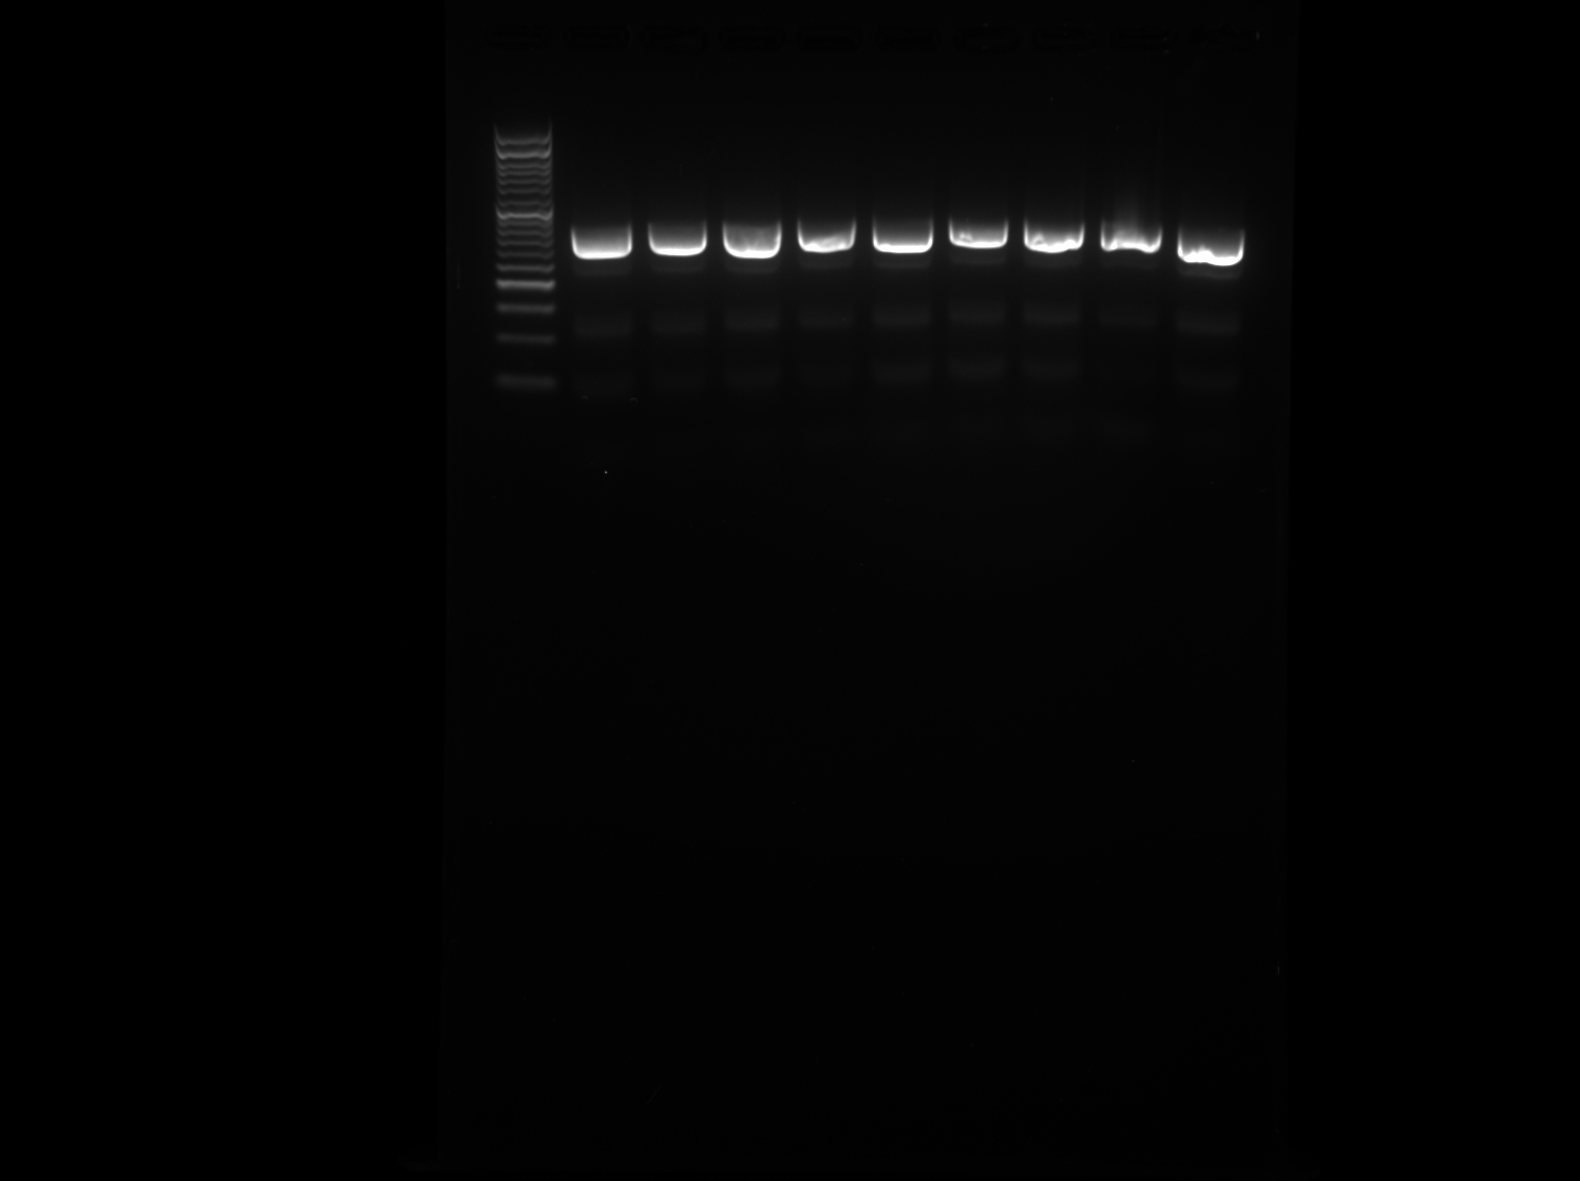
\includegraphics[width=.5\linewidth]{images/gel.png}
  \caption{An example of a successful PCR amplification of the AD template.}
  \label{fig:gel1}
\end{figure}

\bibliographystyle{ieeetr}
\bibliography{main}
\end{document}
